\chapter{Java Messaging Service}

Bei einem klassischen Methoden-Fernaufruf (RMI) ruft der Client eine Methode beim Server auf und wartet auf den Rückgabewert. Dies ist eine synchrone Kommunikation, weil der Client und der Server beide erreichbar sein müssen. Auf Nachrichten basierende Kommunikation ist asynchron, weil der Client und der Server nicht beide verfügbar sein müssen. Durch die lose Kopplung von JMS ergeben sich folgende Vorteile:

\begin{itemize}
	\item Einfache Integration
	\item One-to-many Kommunikation (z.B. Topic-Queue)
	\item Garantierte Lieferung
	\item Transaktionen
\end{itemize}

Die JMS API ist sowohl im EJB Container als auch im Client Container von Java EE vorhanden. In JMS gibt es zwei Architekturen wie Nachrichten versendet werden:

\begin{description}
	\item[Point-to-Point] Die Message-Queue kann mehrere Consumer haben. Wenn einer der Consumer die Message von der Queue konsumiert (liest), dann wird diese gelöscht.
	\item[Publish / Subscribe] Die Topic-Queue hält alle Messages bis sie von allen Subscribern konsumiert wurden. Fällt ein Subscriber aus, behält die Topic-Queue die Message bis der Consumer zurückkommt.
\end{description}

Eine JMS Applikation besteht aus folgenden Bausteinen (siehe Abbildung \ref{fig:jms-overview}):

\begin{figure}
\centering
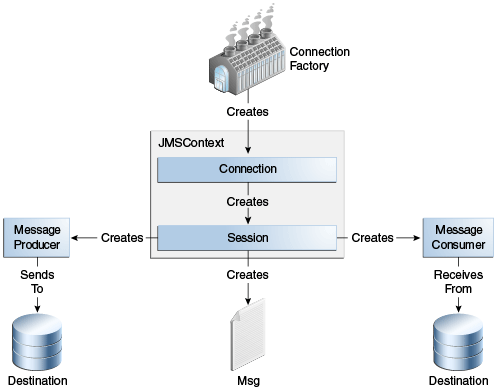
\includegraphics[width=0.7\linewidth]{fig/jms-overview}
\caption{JMS Überblick}
\label{fig:jms-overview}
\end{figure}

\begin{description}
	\item[Administriete Objekte] Dazu gehören die Connection Factories und die Destinations. Beide werden über den Namensdienst (JNDI) angefordert. Die Connection Factory ist für das Erstellen einer Verbindung zuständig un die Destination stellt die Queue zur Verfügung.
	\item[Connection] Eine Connection wird über die Connection Factory hergestellt. Um die Kommunikation zu steuern erstellt die Connection eine Session.
	\item[Session] Aus der Session kann entweder ein Producer oder ein Consumer erstellt werden. Zudem kann sie eine Message erstellen.
	\item[Message Producer] Der Message Producer wird verwendet um eine Message an eine Destination zu senden.
	\item[Message Consumer] Der Message Consumer empfängt Messages aus einer Destination.
	\item[Message] Eine Nachricht welche empfangen oder versendet werden kann. 
\end{description}

Abbildung \ref{fig:send-receive-message} zeigt wie eine Nachricht gesendet bzw. empfangen wird.

\begin{figure}
	\centering
	\begin{subfigure}[b]{0.4\textwidth}
		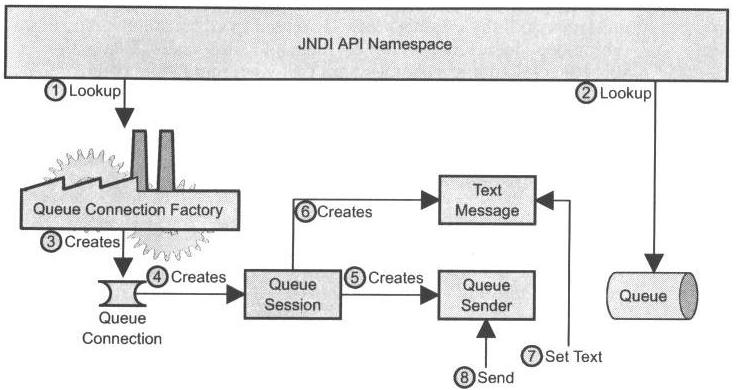
\includegraphics[width=\textwidth]{fig/send-message}
		\caption{Nachricht senden}
	\end{subfigure}
	~
	\begin{subfigure}[b]{0.4\textwidth}
		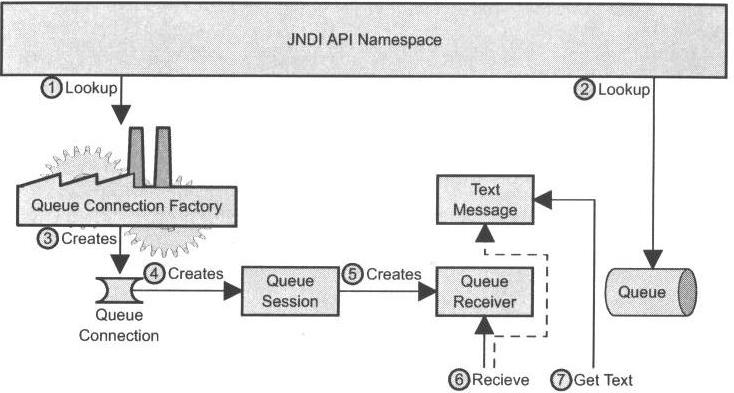
\includegraphics[width=\textwidth]{fig/receive-message}
		\caption{Nachricht empfangen}
	\end{subfigure}
	\caption{Message senden/empfangen}
	\label{fig:send-receive-message}
\end{figure} 


\section{Messages}

Eine Message besteht aus einem Header, den Properties und dem Body. Der JMS Header enthält Informationen über das Routing und die Identifikation. Praktisch alle Felder werden automatisch gesetzt, allerdings kann der Anwender eine Auswahl auch selbst setzen. Die JMS Properties dienen als Ergänzung zu den Header-Feldern. Das JMS API definiert die Property-Namen (z.B. \verb|JMSExpiration|, \verb|JSMPriority|) und die JMS Implementation kann diese unterstützen. Der JMS Body kann mit den folgenden fünf Message Formaten gefüllt werden:

\begin{description}
	\item[StreamMessage:] Ein Stream von primitiven Java Werten wird sequentiell gelesen
	\item[TextMessage:] Ein \verb|String| wird verschickt
	\item[ObjectMessage:] Ein serialisierbares Java Objekt wird verschickt
	\item[ByteMessage:] Uninterpretierte Bytes (binäre Daten) werden verschickt
	\item[MapMessage:] Schlüssel-Werte-Paare werden versendet
\end{description}

Um sicherzustellen das eine Message auch ihr Ziel erreicht gibt es in JMS folgende Mechanismen:

\begin{description}
	\item[Setting time-to-live] Nachricht wird nicht mehr ausgeliefert, falls sie abgelaufen ist
	\item[Specifying message persistence] die Nachricht geht bei Serverausfall nicht verloren
	\item[Controlling acknowledgment] Empfang wird auf verschiedenen Ebenen bestätigt
	\item[Creating durable subscribers] Nachrichten werden über das Pub/Sub-Modell zugestellt
	\item[Setting priorities] Es kann eine Zustell-Priorität (0-9) gesetzt werden
\end{description}

Zudem unterstützt JMS Transaktionen. Der Abschnitt zwischen dem Client und der Queue kann durch eine Transaktion geschützt und bei einem Fehler rückgängig gemacht werden. Listing \ref{lst:transaktionen} zeigt wie eine Transaktion durchgeführt wird.

\begin{lstlisting}[caption=JMS Transaktionen, label=lst:transaktionen]
JMSContext context = connectionFactory.createContext(JMSContext.SESSION_TRANSACTED);
try {
	// send message
	context.commit();
} catch(Exception e) {
	context.rollback();
}
\end{lstlisting}

Wenn ein normaler Consumer erstellt wird, werden so lange Messages empfangen bis der Consumer wieder geschlossen wird. Messages welche eintreffen wenn der Consumer geschlossen ist, werden nicht empfangen (siehe Abbildung \ref{fig:jms-nondurable-subscriber}). Die Session kann aber auch so eingestellt werden, dass die Nachrichten empfangen werden auch wenn der Consumer geschlossen wurde (siehe Abbildung \ref{fig:jms-durable-subscriber}). Dadurch ist eine zuverlässigere Übertragung möglich, was aber auch mehr Overhead erzeugt.

\begin{figure}
	\centering
	\begin{subfigure}[b]{0.4\textwidth}
		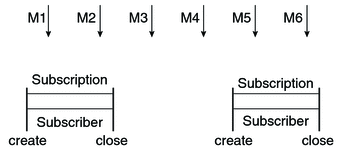
\includegraphics[width=\textwidth]{fig/jms-nondurableSubscriber}
		\caption{Unzuverlässige Client Subscription}
		\label{fig:jms-nondurable-subscriber}
	\end{subfigure}
	~
	\begin{subfigure}[b]{0.4\textwidth}
		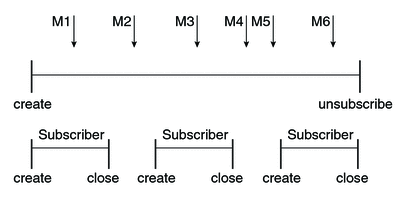
\includegraphics[width=\textwidth]{fig/jms-durableSubscriber}
		\caption{Zuverlässige Client Subscription}
		\label{fig:jms-durable-subscriber}
	\end{subfigure}
	\caption{Client Subscription}
\end{figure} 

\section{Message Driven Beans (MDB)}

Message Driven Beans (\verb|@MessageDriven|) erlaubt es einer Java EE Applikation asynchron Messages zu konsumieren (EJB kommunizieren synchron). Jedes Bean (Stateless, Session, Message Driven) kann synchron Messages als Producer versenden. Es kann auch jedes Bean Messages synchron empfangen, allerdings ist dies nicht empfohlen, weil man dadurch an den Sender gekoppelt ist. Deshalb sollten besser asynchrone Empfänger verwendet werden. In einem Session Bean würde sich das mit einer \verb|@Async|-Methode realisieren lassen, aber man sollte die MDB verwenden da diese speziell dafür gedacht sind.

MDB sind ähnlich zu Stateless Beans, halten also keine Daten oder Status für einen Client. Alle Instanzen eines MDBs sind gleichwertig. Der Container kann die Nachricht an jedes MDB weitergeben. MDB werden asynchron ausgeführt sobald eine Nachricht eintrifft und sind kurzlebig. Abbildung \ref{fig:mdb-lifecycle} zeigt den Life Cycle eines MDB.

\begin{figure}
\centering
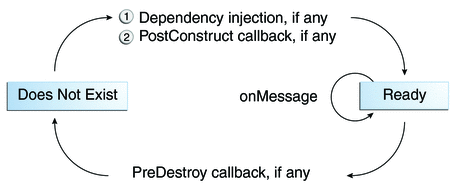
\includegraphics[width=0.7\linewidth]{fig/mdb-lifecycle}
\caption{MDB Life Cycle}
\label{fig:mdb-lifecycle}
\end{figure}


\section{Kontrollfragen}